\documentclass[conference]{IEEEtran}
\IEEEoverridecommandlockouts

% Plantilla armada por Agustín (2/11). SOLO estructura, tablas de datos y figuras:
% la letra prohíbe usar IA para redactar el informe, así que todo el texto lo
% escribimos nosotros donde dice "REDACTAR". Compilar en Overleaf (pdfLaTeX).

\usepackage{iftex}
\ifPDFTeX
  \usepackage[T1]{fontenc}
  \usepackage[utf8]{inputenc}
\else
  \usepackage{fontspec}
\fi
\usepackage[spanish,es-tabla]{babel}

\usepackage{cite}
\usepackage{amsmath,amssymb,amsfonts}
\usepackage{graphicx}
\usepackage{booktabs}
\usepackage{textcomp}
\usepackage{xcolor}

% Marcador visible para lo que falta escribir. Antes de entregar: buscar "REDACTAR"
% y verificar que no quede ninguno.
\newcommand{\redactar}[1]{\textcolor{red}{[REDACTAR: #1]}}

\begin{document}

\title{Aterrizaje lunar con Deep Q-Networks: implementación, análisis de la política y estudio de ablación}

\author{
\IEEEauthorblockN{Thiago Rivas}
\IEEEauthorblockA{C.I. 5.475.680-3 \\
\textit{Facultad de Ingeniería} \\
\textit{Universidad de la República}\\
Montevideo, Uruguay \\
thiago.rivas0021@gmail.com}
\and
\IEEEauthorblockN{Juan Duarte}
\IEEEauthorblockA{C.I. 5.201.302-9 \\
\textit{Facultad de Ingeniería} \\
\textit{Universidad de la República}\\
Montevideo, Uruguay \\
juan.duarte@fing.edu.uy}
\and
\IEEEauthorblockN{Agustin Occhiuzzi}
\IEEEauthorblockA{C.I. 5.480.562-4 \\
\textit{Facultad de Ingeniería} \\
\textit{Universidad de la República}\\
Montevideo, Uruguay \\
agustin.occhiuzzi@fing.edu.uy}
}

\maketitle

% =========================================================
% PRESUPUESTO DE ESPACIO: límite duro de 5 páginas en total (2 columnas, 10pt).
% ~1000 palabras por página de solo texto. Con 2 tablas y 3 figuras quedan
% unas 3000 palabras. Reparto sugerido:
%   Resumen 150 | Introducción 250 | DQN (a) 500 | Calibración (b) 350
%   Aprendizaje y desempeño (c) 400 | Política (d) 500 | Ablación (e) 600
%   Limitaciones y conclusiones 250
% Responsables (plan 2/11): Thiago -> II y III; Fran -> VI; Agustín -> V y VII.
% =========================================================

\begin{abstract}
\redactar{problema, método, resultado principal (tasa de éxito del completo) y
conclusión de la ablación, en 4 a 6 oraciones}
\end{abstract}

\begin{IEEEkeywords}
aprendizaje por refuerzos, DQN, LunarLander, ablación
\end{IEEEkeywords}

\section{Introducción}
\redactar{el problema LunarLander-v3 (estado de 8 dimensiones, 4 acciones, éxito
$R \geq 200$), el objetivo de superar 10\% de éxito y la estructura del artículo}

% ---------------------------------------------------------
\section{Solución DQN implementada}   % letra (a) — Thiago
\label{sec:dqn}
\redactar{red Q, memoria de repetición, red objetivo, $\varepsilon$-greedy, pérdida
de Huber; diferencias con Mnih et al.~\cite{mnih2015}; manejo de terminado vs.\ truncado}

% Ecuación del objetivo, por si se usa:
% \begin{equation}
% y = r + \gamma\,(1-d)\max_{a'} Q(s',a';\theta^-)
% \end{equation}

\begin{table}[htbp]
\caption{Configuración de referencia (A0)}
\label{tab:hiper}
\centering
\begin{tabular}{@{}ll@{}}
\toprule
Hiperparámetro & Valor \\
\midrule
Red Q & MLP $8 \to 64 \to 64 \to 4$, ReLU \\
Optimizador & Adam, $\text{lr} = 10^{-3}$ \\
Descuento $\gamma$ & 0,99 \\
Memoria / minilote & 50\,000 / 64 (muestreo uniforme) \\
Inicio del aprendizaje & 1\,000 pasos \\
Actualización & cada 4 pasos \\
Red objetivo & copia cada 1\,000 pasos \\
Exploración & $\varepsilon$: 1 $\to$ 0,05 lineal en 200 episodios \\
Pérdida & Huber ($\beta=1$), norma del gradiente $\leq 10$ \\
Presupuesto & 300 episodios de hasta 1\,000 pasos \\
\bottomrule
\end{tabular}
\end{table}

% ---------------------------------------------------------
\section{Selección de hiperparámetros}   % letra (b) — Thiago
\redactar{cómo se llegó a A0: comparaciones de dos configuraciones por persona
(arquitectura y lr; replay y minilote; esquema de exploración), sin búsqueda grande.
Evidencia del foco C: con 5 semillas y 600 episodios, $\varepsilon$ por episodios
(exponencial) alcanzó 177 de recompensa media contra 127 del lineal por pasos
(diferencia no significativa, $p=0{,}22$), porque el lineal deja de explorar hacia el
episodio 220. Ver \texttt{AgustinAgente/EXPLICACION\_AgenteDQN.md}, sec.~9.3}

% ---------------------------------------------------------
\section{Aprendizaje y desempeño final}   % letra (c) — Thiago/Fran
\redactar{curva de aprendizaje (figura de Thiago), evaluación greedy en 200 episodios
(semillas 10000--10199) de las 8 semillas del completo, comparación con el agente
aleatorio; protocolo de semillas de entrenamiento y evaluación}

% \begin{figure}[htbp]
% \centerline{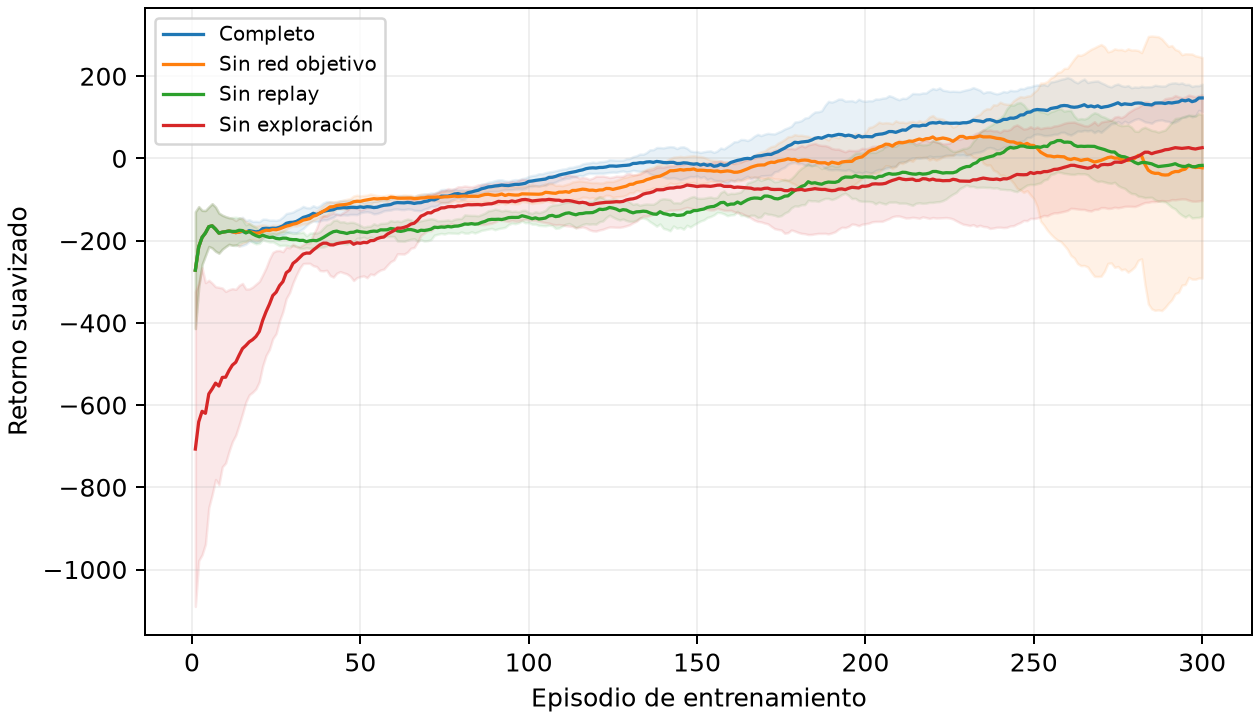
\includegraphics[width=\columnwidth]{figuras/curvas_aprendizaje.png}}
% \caption{...}
% \label{fig:curvas}
% \end{figure}

% ---------------------------------------------------------
\section{Análisis de la política}   % letra (d) — Agustín
\label{sec:politica}
% Material: TAREA2/analisis_politica/ (figuras y metricas_politica.json) y la
% sección 13 de AgustinAgente/EXPLICACION_AgenteDQN.md (lectura de cada figura).
\redactar{método: cortes que varían dos dimensiones del estado con las otras seis
fijas ($x=0$, $y=0{,}8$, $v_x=0$, $v_y=-0{,}3$, $\theta=\omega=0$, sin contacto),
con los estados visitados superpuestos porque los estados sintéticos pueden no ser
alcanzables}

\begin{figure*}[htbp]
\centerline{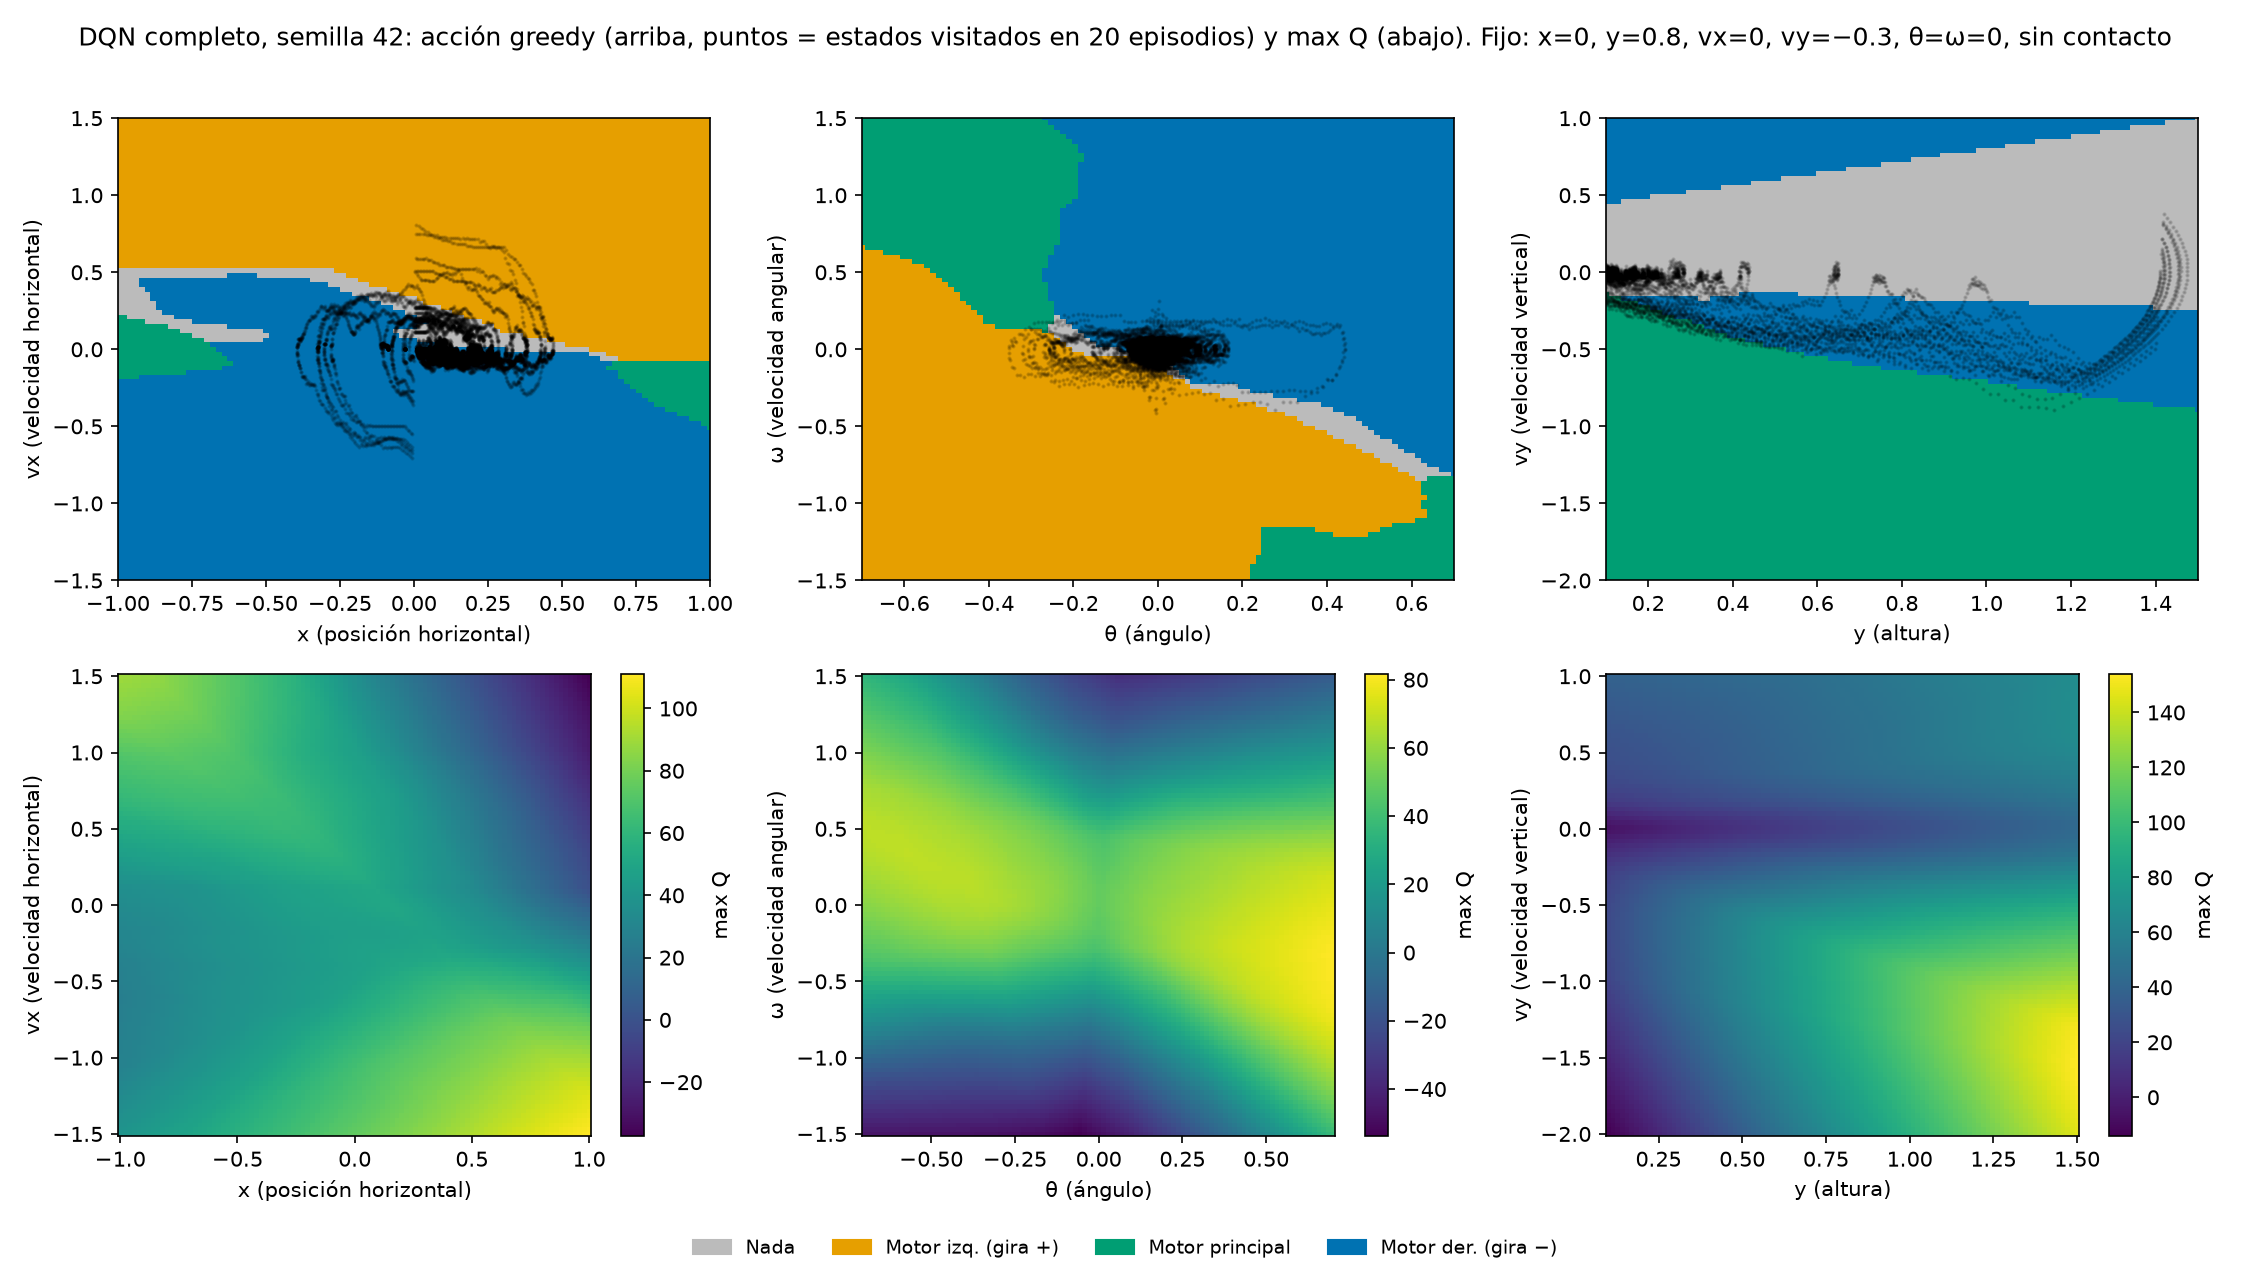
\includegraphics[width=\textwidth]{figuras/cortes_completo_s42.png}}
\caption{\redactar{epígrafe: DQN completo, semilla 42; acción greedy (arriba) y $\max_a Q$ (abajo)}}
\label{fig:cortes}
\end{figure*}

\redactar{qué muestra cada corte: (1) altura--$v_y$: motor principal por debajo de una
frontera que baja con la altura (frena antes cuanto más cerca del suelo);
(2) ángulo--velocidad angular: el motor lateral se elige según el signo de $\omega$,
desplazado por $\theta$ (contrarresta el giro); (3) $x$--$v_x$: corrige la deriva
horizontal, pero no es simétrico}

\begin{figure}[htbp]
\centerline{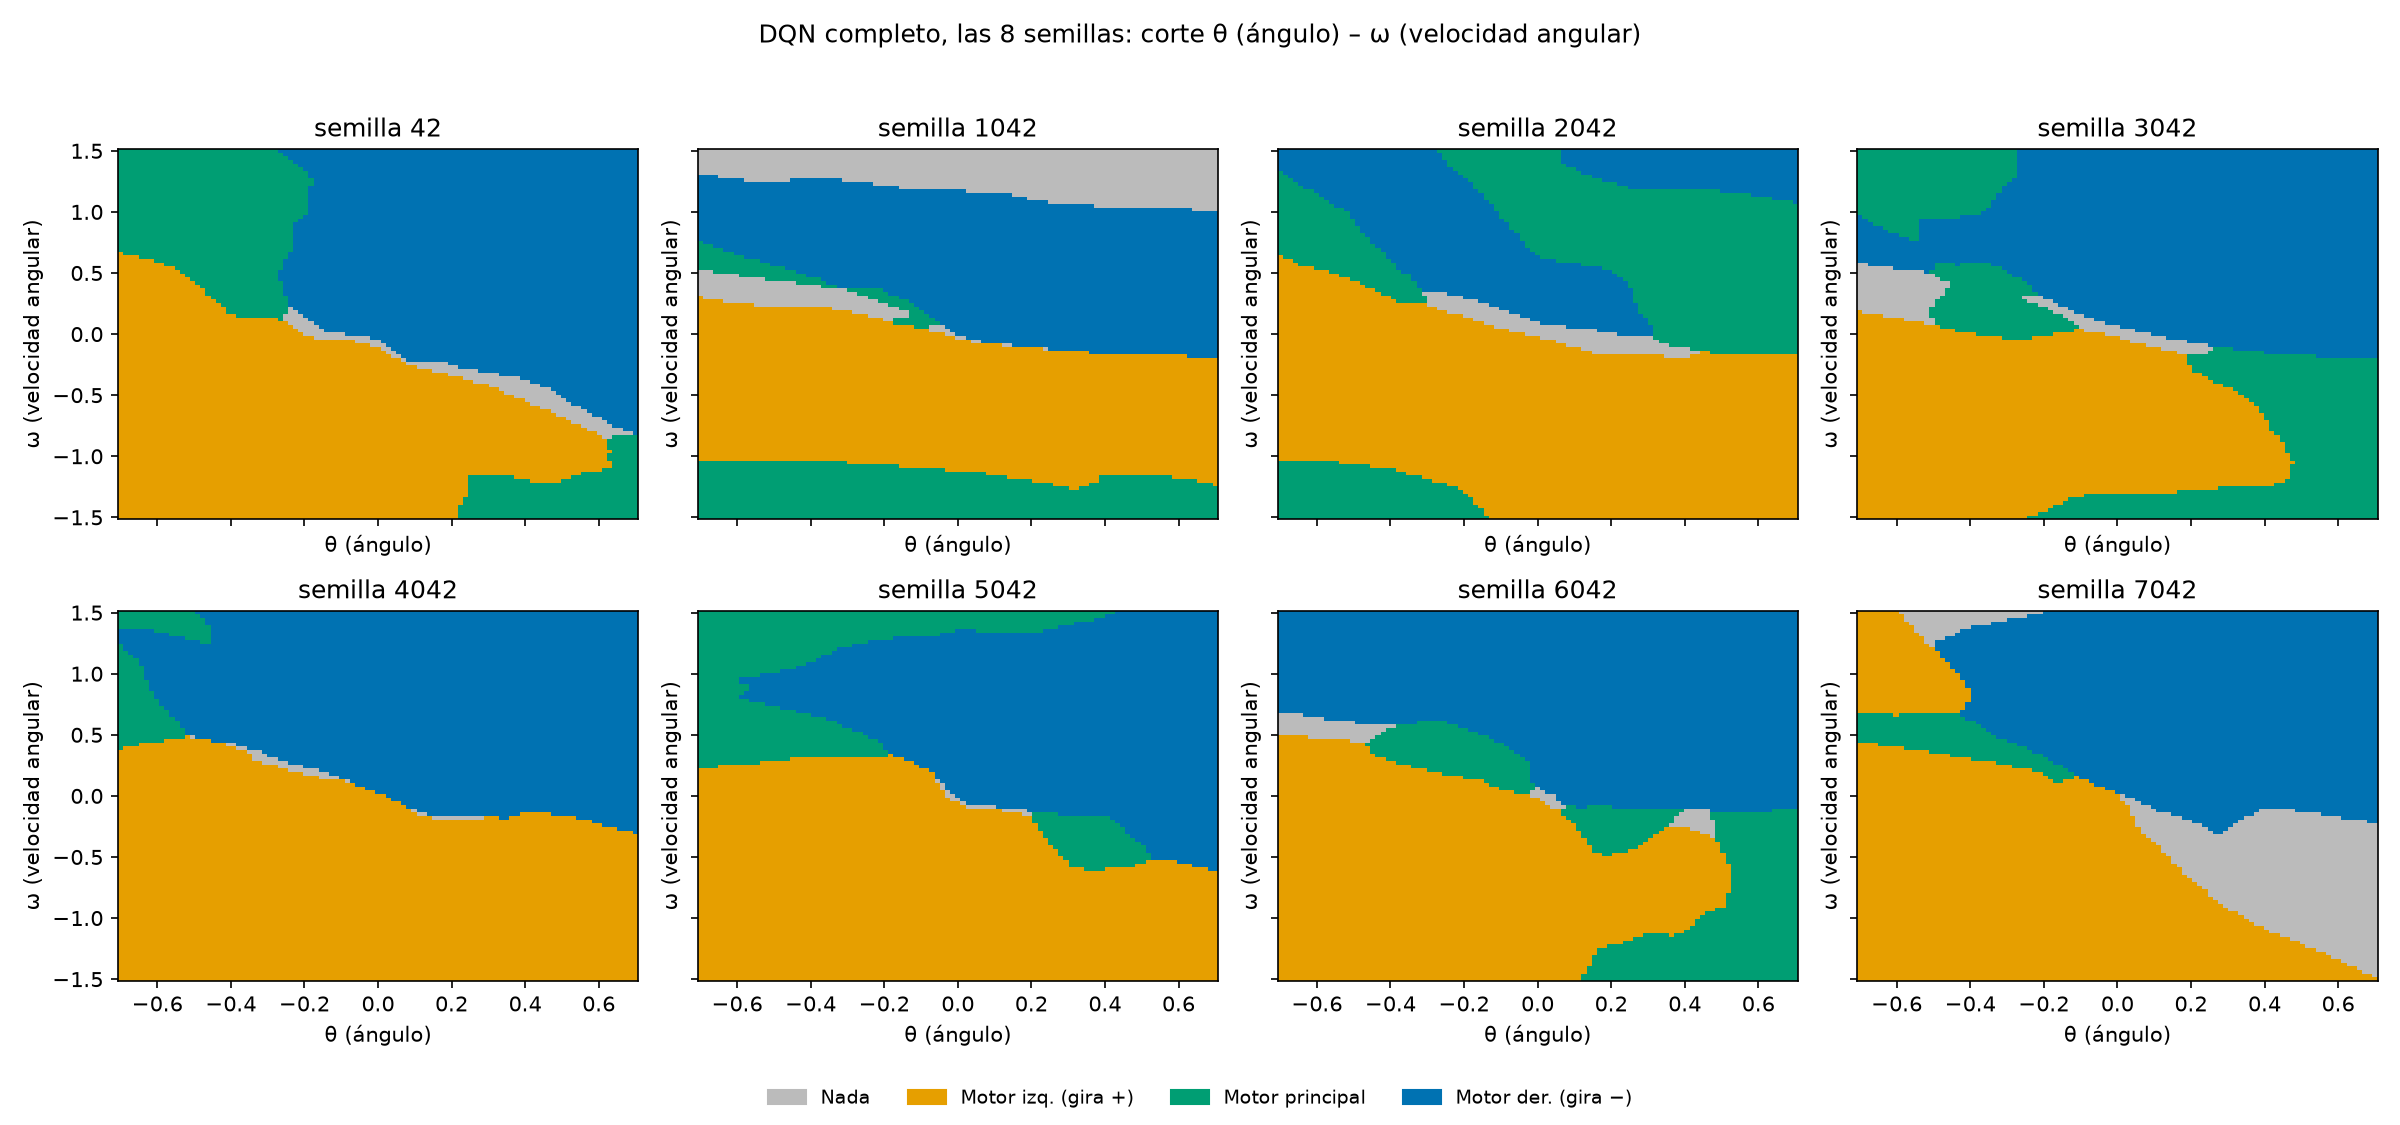
\includegraphics[width=\columnwidth]{figuras/cortes_8_semillas_angulo.png}}
\caption{\redactar{epígrafe: el corte ángulo--$\omega$ en las 8 semillas}}
\label{fig:semillas}
\end{figure}

\redactar{qué es estable entre semillas (regla de $\omega$ en las 8) y qué cambia
(regiones de motor principal y de ``nada''); cómo terminan los episodios: los fracasos
del completo son casi siempre flotar hasta el paso 1000, no choques}

\begin{table}[htbp]
\caption{Cómo terminan 20 episodios greedy (semillas 10000--10019), suma de las 8 semillas}
\label{tab:fines}
\centering
\begin{tabular}{@{}lrrr@{}}
\toprule
Variante & Posa & Choca & Flota (1000 pasos) \\
\midrule
Completo & 101 & 7 & 52 \\
Sin exploración & 35 & 49 & 76 \\
Sin replay & 23 & 135 & 2 \\
Sin red objetivo & \multicolumn{3}{c}{pendiente} \\
\bottomrule
\end{tabular}
\end{table}

% Figura opcional si sobra espacio: figuras/acciones_por_altura.png o
% figuras/cortes_completo_vs_sin_exploracion.png

% ---------------------------------------------------------
\section{Estudio de ablación}   % letra (e) — Fran
\redactar{variantes (sin red objetivo, sin replay con minilote efectivo 1, sin
exploración con $\varepsilon=0$), 8 semillas por condición, misma evaluación;
test: U de Mann--Whitney bilateral exacto~\cite{mann1947} sobre las 8 medias por
condición, corrección de Holm~\cite{holm1979} por 3 comparaciones, $\alpha=0{,}05$;
Wilcoxon emparejado como análisis de sensibilidad; conclusiones}

\begin{table}[htbp]
\caption{Recompensa media de evaluación por condición (8 semillas)}
\label{tab:ablacion}
\centering
\begin{tabular}{@{}lrrrr@{}}
\toprule
Condición & Media & Dif. & $p$ MW & $p$ Holm \\
\midrule
Completo & 137,8 & --- & --- & --- \\
Sin red objetivo & \multicolumn{4}{c}{pendiente (Thiago)} \\
Sin replay & $-0{,}8$ & $-138{,}7$ & 0,007 & \textit{(*)} \\
Sin exploración & 25,8 & $-112{,}0$ & 0,065 & \textit{(*)} \\
\bottomrule
\multicolumn{5}{@{}l}{\footnotesize (*) Holm se calcula cuando estén las tres comparaciones.}
\end{tabular}
\end{table}

% ---------------------------------------------------------
\section{Limitaciones}   % Agustín
\redactar{8 semillas: potencia limitada (MW con 8 contra 8); 300 episodios: los agentes
siguen mejorando; corridas en máquinas y versiones de torch distintas no son
reproducibles bit a bit; evaluación en semillas de desarrollo (10000--10199) también
usadas para ajustar; cortes en estados sintéticos; sin replay depende de la
definición elegida (minilote 1)}

\section{Conclusiones}
\redactar{}

\section*{Uso de Inteligencia Artificial}
\redactar{declarar el uso de IA en el código y que el informe fue redactado por el
equipo (la IA solo se usó para corrección gramatical, si corresponde)}

\begin{thebibliography}{00}
\bibitem{mnih2015} V.~Mnih \textit{et al.}, ``Human-level control through deep
reinforcement learning,'' \textit{Nature}, vol.~518, pp.~529--533, 2015.
\bibitem{sutton2018} R.~S.~Sutton y A.~G.~Barto, \textit{Reinforcement Learning: An
Introduction}, 2.\textsuperscript{a} ed. Cambridge, MA, USA: MIT Press, 2018.
\bibitem{towers2024} M.~Towers \textit{et al.}, ``Gymnasium: A standard interface for
reinforcement learning environments,'' arXiv:2407.17032, 2024.
\bibitem{mann1947} H.~B.~Mann y D.~R.~Whitney, ``On a test of whether one of two random
variables is stochastically larger than the other,'' \textit{Ann. Math. Statist.},
vol.~18, no.~1, pp.~50--60, 1947.
\bibitem{holm1979} S.~Holm, ``A simple sequentially rejective multiple test procedure,''
\textit{Scand. J. Statist.}, vol.~6, no.~2, pp.~65--70, 1979.
\end{thebibliography}

\end{document}
